\documentclass[l4proj.tex]{subfiles}
\begin{document}    

This chapter will look into the agile project management concepts the RViT is built upon and then examine the positive and negative aspects of market-leading agile project management tools.

\section{Agile project management}
Agile methodology support is at the core of any project management tool designed for agile teams.

\subsection{Requirement Identification and the role of Epics and User Stories}
The majority of requirements are developed into epics and user stories. Good user story practices is crucial to efficient software development. User story templates can be used to aid teams in writing user stories. Definition of dones provide developers with a succinct explanation to compare their development to.

User story points can allow teams to effectively manage workloads and estimate how long particular tasks will take - talk about different types of . Category tags allow developers to know what types of development certain tasks will require, allowing for streamlines user assignment.

Pair and mob programming support to allow for multiple users to work on one story at once. Priority options can help teams to prioritise stories, restricted range to limit confusion. 

Epic and user story mapping allows for developers to understand which story belongs to each epic. By being able to reorder these elements, developers can visually prioritise epics and user stories without having to use extremely fine-grained priority choices.

\subsection{Visualising Project Progress}
It is important for teams to be able to visualise their progress to allow for further prioritisation. Most modern approaches to this are based on the Kanban flow developed by Toyota [ref]. This was originally used in lean manufacturing but its applications were far reaching allowing for the kanban method to be born. 

While not as popular as the scrum methodology, kanban comes in second [stats and ref]. Kanban was chosen as a base for this project as it allows for future scrum based development.

Kanban boards and WIP limits can help agile teams identify bottlenecks and blockers in their work and are often essential in stand-up meetings. 

\subsection{The Importance of Visible Business Value}
What is a business value and why should developers care about them?

Epics and user stories typically have business value associated with them, however development teams and project stakeholders are often unaware of these at a glance [Peggy's research]. 

While a good user story should explain the business value of the task, it would be beneficial to be able to understand the value a epic or user story brings at a glace.

By defining a subset of business values, custom to a particular agile team, these can be used on epics and user stories to allow for a quick, streamlined value identification process. By making it easy for developers to identify business values it is also hoped that these will be taken into consideration during the prioritisation process and become a more integral part of an agile team's workflow. 

Highlighting the business value of an epic or user story will also help developers understand the purpose behind a particular task hopefully increasing knowledge surrounding the utility cost of the task and increasing developer motivation [expectancy value theory]. 

\section{Existing Products}
There are many pre-existing agile project management tools on the market with considerable funding and industry backing. This selection provides a review of three of the industry leading tools, identifying the strengths and weaknesses of each and explaining were RViT finds its niche among competitors.


\subsection{Jira}
Jira is a state-of-the-art project management tool, servicing over 65,000 companies across the globe \cite{JiraUsers}. The tool offers extensive customisation options and supports a variety of agile methodologies including scrum and kanban, as seen in Figure \ref{fig:Jira kanban}.
Jira also provides out-of-the-box metric reporting including burndown and velocity charts as well as cumulative flow diagrams \cite{JiraReports}. Atlassian Open DevOps also automatically connects Jira with any of Atlassian's partner tools such as GitHub and BitBucket without the traditional overhead \cite{JiraDevOps}. Jira also provides extensive documentation. 

\begin{figure}[h!]
\begin{center}
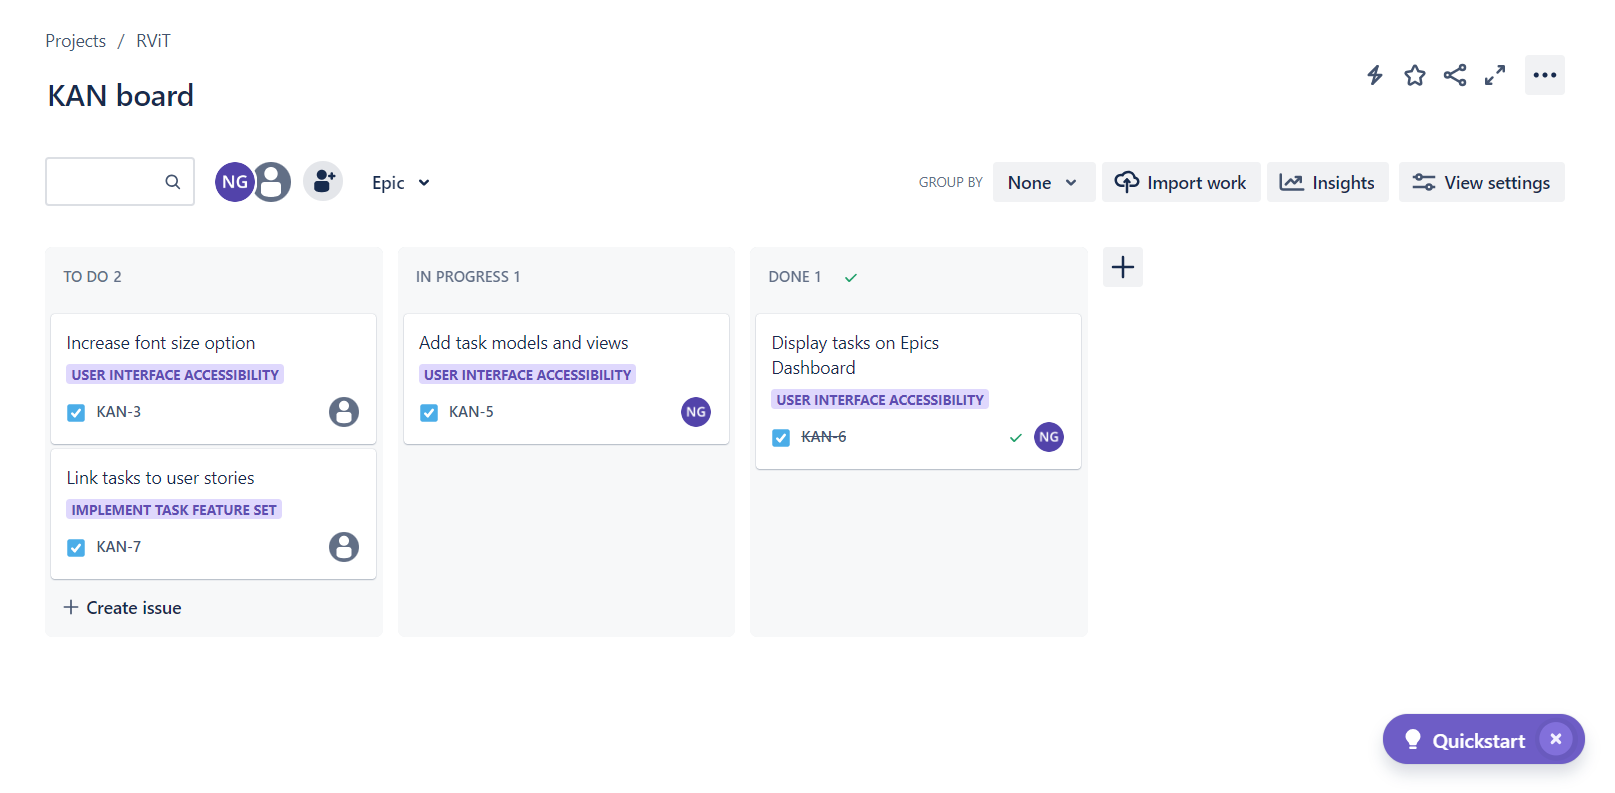
\includegraphics[scale=0.35]{dissertation/images/JiraKanbanBoard.png}
\caption{Example Jira kanban board}
\label{fig:Jira kanban} 
\end{center}
\end{figure}

As Jira is part of the Atlassian software set, the Atlassian Market place provides additional third-party Jira plug-ins and integrations to allow agile teams to further personalise their experience.  

One of the common criticisms of Jira is that the number of features it supports can be overwhelming for unfamiliar users and leads to a steep learning curve \cite{JiraProblemsFeatures}. The amount of customisability can also be a problem with teams sometimes creating unintuitive dashboard with too many fields to fill out \cite{JiraProblemsFlexible}. Jira is also only free to use for teams of up to 10 developers, with a slightly limited feature set. RViT aims to combat these issues by providing a free-to-use streamlined approach to kanban development that cuts out unnecessary overhead and aims to provide an easy to use Jira alternative. 


\subsection{Trello}
Trello is another Atlassian project management tool, though unlike Jira it has a significantly reduced feature set, focusing on kanban methodology support as seen in Figure \ref{fig:Trello kanban}. Another difference to Jira, is Trello is pitched as a general project management tool as opposed to an agile one. This means typical agile methodology support such as creating epics is not present in Trello.

Similarly to Jira, Trello also has its own marketplace where you can add third party extensions called 'power-ups'. Power-ups can be anything from adding a priority component to your story to adding GitHub integration.

Trello is user friendly and intuitive to use with many example templates to quick start a board. However, the free version only supports the kanban board itself and not any of the other views such as the dashboard or calendar view \cite{TrelloPricing}. RViT plans to create a similarly intuitive interface but with more out of the box agile methodology support such as allowing users to create epics, define definitions of done, and add clear tags, values and priorities.


\begin{figure}[h!]
\begin{center}
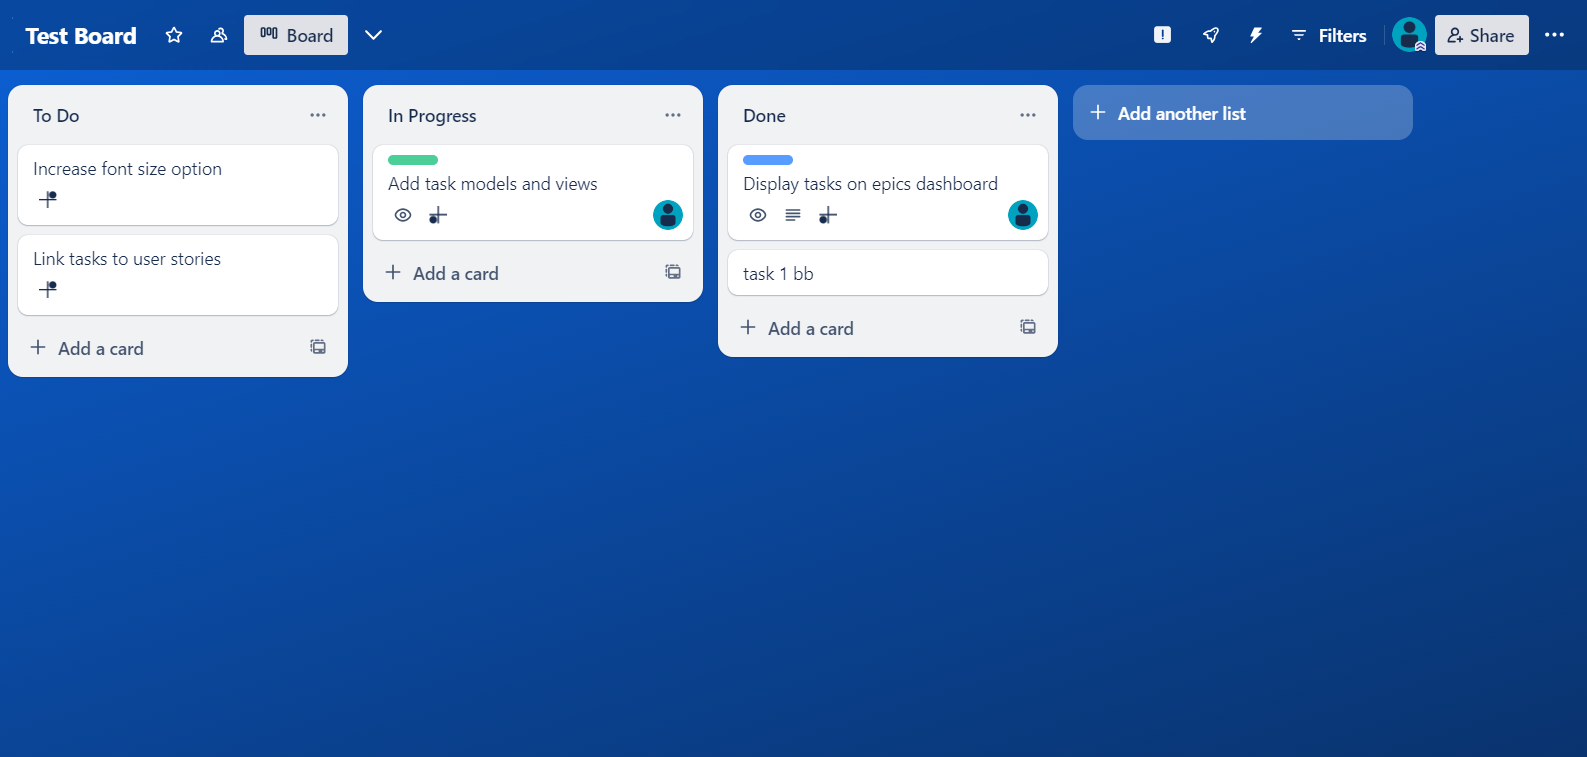
\includegraphics[scale=0.35]{dissertation/images/TrelloKanbanBoard.png}
\caption{Example Trello kanban board}
\label{fig:Trello kanban} 
\end{center}
\end{figure}
]]

\subsection{GitHub Issues and Projects}
GitHub has built in issue tracking support. Users can define issues and create custom issue templates to simplify the issue adding process. GitHub also allows developers to add customisable labels to a project and define milestones to add support for scrum-based teams. GitHub issues and projects are also accessible from the GitHub repository itself, meaning a secondary application does not have to be used. The tools are also completely free to use unlike Jira and Trello.

GitHub projects support three different views of a repository's issues, a kanban board-based, a table-based and a roadmap-based view. These views are intuitive to use but are not very visually appealing due to the lack of colour as seen in Figure \ref{fig:GitHub kanban}. As well as this, the information that a developer can gain without clicking into an issue is limited with there being no priority support and any labels the issue has not being visible until the issue is clicked into.

\begin{figure}[h!]
\begin{center}
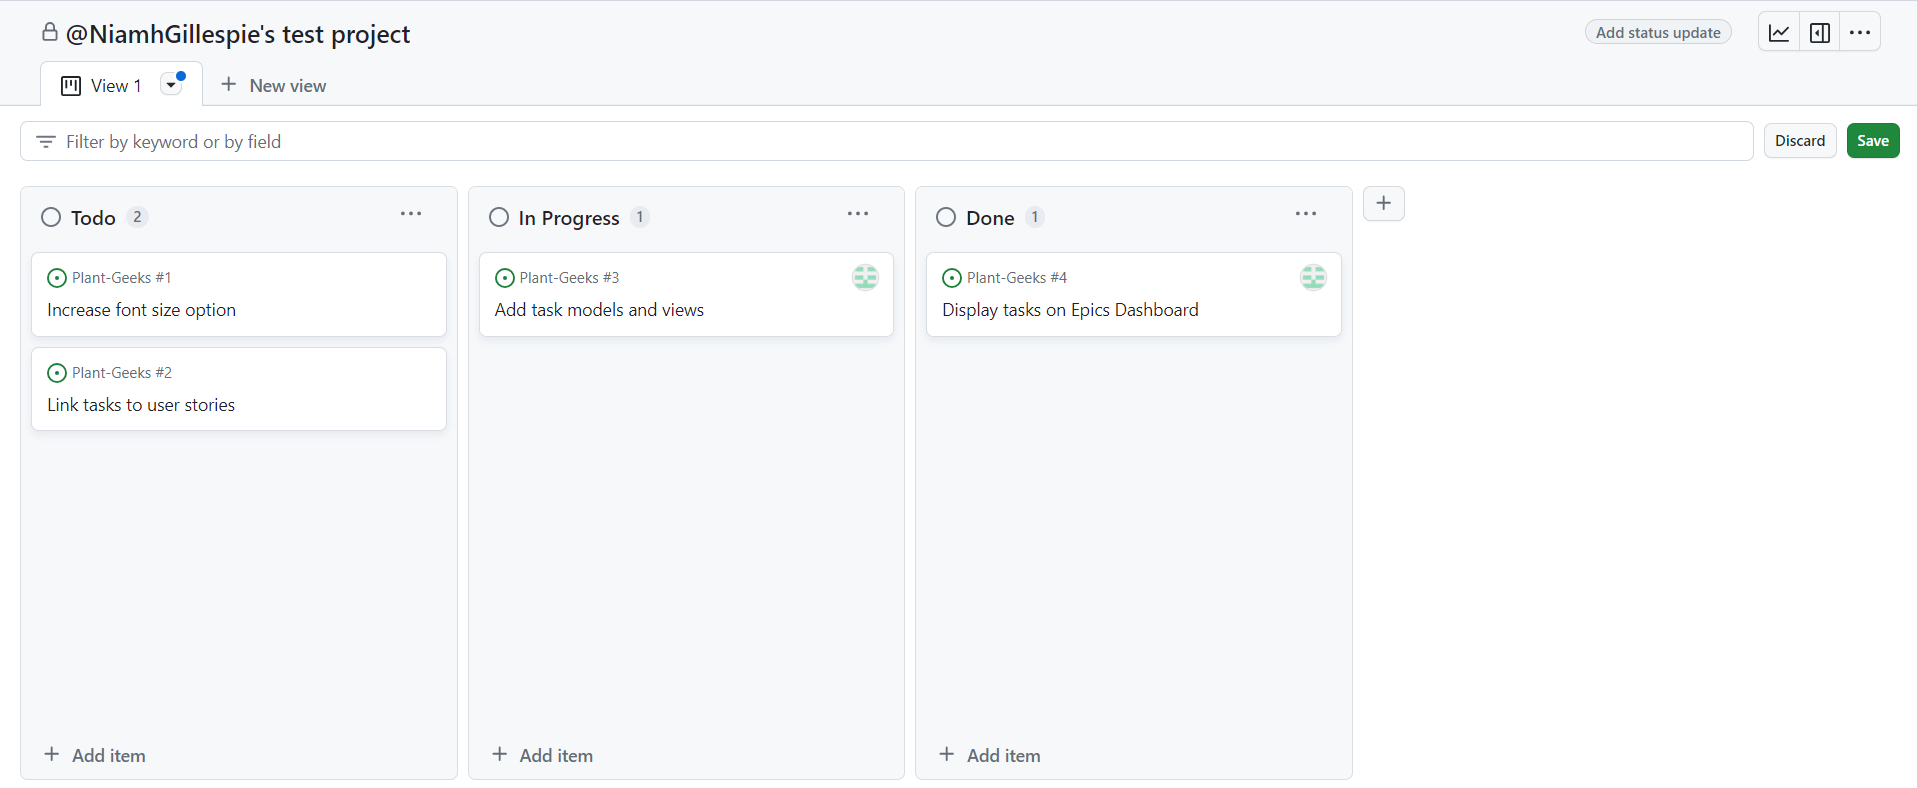
\includegraphics[scale=0.35]{dissertation/images/GitHubKanbanBoard.png}
\caption{Example GitHub kanban board}
\label{fig:GitHub kanban} 
\end{center}
\end{figure}
]]

Like Trello, GitHub also lacks support for agile concepts like epics. RViT aims to support these concepts while also providing a more aesthetically pleasing user interface. 

\end{document}